\documentclass[english, version-2020-11]{uzl-thesis}
\UzLStyle{pagella contrast design}
\usepackage{comment}
\usepackage{float}
\lstset{basicstyle=\ttfamily}
\usepackage{tikz}
\usetikzlibrary{shapes.geometric, arrows.meta, positioning, shadows.blur}

\tikzstyle{process} = [
    rectangle, rounded corners,
    minimum width=4.2cm,
    minimum height=1.2cm,
    text centered,
    draw=black,
    fill=blue!10,
    font=\sffamily\small,
    blur shadow
]

\tikzstyle{arrow} = [
    thick,
    ->,
    >=Stealth,
    draw=gray!80
]

\tikzstyle{cell} = [rectangle, draw=black, minimum width=2.5em, minimum height=2.5em, anchor=center]
\tikzstyle{native} = [cell, fill=blue!20]
\tikzstyle{enclave} = [cell, fill=red!20]
\tikzstyle{label} = [font=\bfseries]


\UzLThesisSetup{
Masterarbeit,
Verfasst              = {am}{Institut für Technische Informatik},
Titel auf Deutsch     = {
    Bewertung von RISC-V-Enklaven: Leistungsbenchmarks und bewährte Konfigurationspraktiken
}, 
Titel auf Englisch    = {
    Evaluating RISC-V Enclaves: Performance Benchmarks and Configuration Best Practices 
},
Autor                 = {Basil Ugbomoiko},
Betreuerin            = {Dr.-Ing. Saleh Mulhem},
Mit Unterstützung von = {Henrik Strunck, M.Sc},
Studiengang           = {IT Security},
Datum                 = {31. August 2025},
Abstract = {This thesis evaluates the performance of Keystone enclaves, an open-source Trusted Execution Environment (TEE) designed for RISC-V platforms. Keystone enables secure computation by isolating sensitive workloads from the rest of the system. To assess its performance, the study benchmarks critical system parameters, including the number of CPU cores, cache size, memory allocation, and enclave configuration. Using industry-standard benchmarking tools such as Dhrystone and CoreMark, the research measures execution time, context switch overhead, memory latency, and CPU utilization across a range of hardware and software configurations. The experimental analysis identifies key performance bottlenecks that impact the efficiency of enclave execution. Based on these findings, the study presents configuration best practices and tuning recommendations tailored to various workload profiles, such as compute-bound, memory-intensive, and mixed applications. The insights gained from this evaluation contribute to optimizing the deployment of Keystone enclaves, making them more viable for real-world use cases that demand secure and efficient execution on RISC-V architectures.},
Zusammenfassung = {Diese Arbeit bewertet die Leistung von Keystone-Enklaven, einer Open-Source Trusted Execution Environment (TEE) für RISC-V-Plattformen. Keystone ermöglicht sichere Berechnungen, indem sensible Workloads vom restlichen System isoliert werden. Zur Leistungsbewertung werden zentrale Systemparameter wie die Anzahl der CPU-Kerne, die Cache-Größe, die Speicherzuweisung und die Konfiguration der Enklave untersucht. Mithilfe standardisierter Benchmarking-Tools wie Dhrystone und CoreMark werden Ausführungszeit, Kontextwechsel-Overhead, Speicherlatenz und CPU-Auslastung unter verschiedenen Hardware- und Softwarekonfigurationen gemessen. Die experimentelle Analyse identifiziert wichtige Leistungsengpässe, die die Effizienz der Enklaven beeinträchtigen. Auf Basis dieser Erkenntnisse werden Konfigurationsrichtlinien und Optimierungsempfehlungen vorgestellt, die auf unterschiedliche Workload-Profile zugeschnitten sind, z. B. rechenintensive, speicherintensive und gemischte Anwendungen. Die gewonnenen Erkenntnisse tragen dazu bei, den Einsatz von Keystone-Enklaven zu optimieren und ihre praktische Anwendbarkeit in sicherheitskritischen Bereichen auf RISC-V-Architekturen zu verbessern.},
Numerische Bibliographie
} % Put your \UzLStyle and \UzLThesisSetup here
\addbibresource{refs.bib}

\begin{document}

%\chapter{Introduction}

\section{Contributions of this Thesis}
This thesis makes several substantive contributions to the study and evaluation of Trusted Execution Environments (TEEs), with a particular emphasis on the Keystone framework. The research spans architectural analysis, emulation-based deployment, and empirical performance evaluation. The primary contributions are enumerated below:

\begin{itemize}
\item \textbf{Comprehensive Architectural Analysis of Keystone:}
The thesis presents a detailed and systematic examination of the Keystone TEE framework. This includes an in-depth discussion of its core architectural elements, such as the Security Monitor (SM), enclave runtime environment, and user-level application design. The role of RISC-V’s privilege hierarchy and Physical Memory Protection (PMP) in enforcing strict isolation guarantees is elaborated, thereby providing a holistic view of Keystone’s security architecture.
\item \textbf{Comparative Evaluation with Established TEEs:}  
A comparative study is conducted to evaluate Keystone alongside widely deployed commercial TEEs, namely Intel Software Guard Extensions (SGX) and ARM TrustZone. This analysis investigates fundamental architectural distinctions, including enclave creation models, privilege separation strategies, scalability, TCB size, and extensibility. The comparison helps contextualize Keystone’s design philosophy and clarifies its advantages in terms of openness and modularity.

\item \textbf{Virtualized Deployment and Toolchain Integration:}  
The thesis demonstrates the practical deployment of Keystone in a fully virtualized environment using a RISC-V-specific fork of the QEMU emulator. This setup facilitates development and testing without the need for physical RISC-V hardware. It also documents the toolchain configuration, build process, and debugging workflow, thereby offering a reproducible methodology for future research and evaluation.

\item \textbf{Performance Evaluation Using Synthetic Benchmarking:}  
To assess the runtime impact of enclave-based execution, Keystone enclaves are benchmarked using two widely accepted synthetic workloads: Dhrystone and CoreMark. The thesis measures key performance indicators—including execution time, Dhrystones per second (DMIPS), iterations per second (IPS), and standard deviation across runs—to quantify the overhead introduced by enclave isolation and security enforcement.

\item \textbf{Workload Characterization Under Enclave Constraints:}  
The computational behavior of the benchmark applications is analyzed in the context of enclave execution. The findings provide empirical insight into how TEE-induced isolation affects instruction throughput and memory interaction patterns, thus illustrating the performance-security trade-offs inherent to enclave-based models.
\end{itemize}

\section{Related Work}

The field of Trusted Execution Environments has been shaped by a combination of commercial deployments and academic proposals, each addressing different aspects of secure computing. This section situates the present work within the broader landscape of TEE research and implementation.

Intel SGX is one of the most well-known commercial TEE solutions. It introduces user-space enclaves with hardware-enforced isolation and memory encryption. SGX supports fine-grained protection mechanisms and remote attestation, making it suitable for confidential computing scenarios. However, SGX is hindered by several limitations, including rigid enclave memory constraints, lack of supervisor-mode support, and a closed-source implementation that precludes low-level architectural exploration or modification. These issues restrict its applicability in research and experimental systems development.

ARM TrustZone represents a different paradigm, based on the separation of execution into a Secure World and a Normal World. While TrustZone enables trusted operating systems and supports a variety of secure services, it suffers from scalability issues, particularly in multi-core environments where interrupt handling becomes a bottleneck. Moreover, TrustZone's coarse-grained isolation and reliance on a monolithic Secure World kernel contribute to a large TCB, which poses challenges for security assurance and formal verification.

In the academic domain, projects such as Sanctum and Sancus have contributed lightweight and formally verifiable secure execution frameworks. Sanctum builds on RISC-V to enforce secure memory isolation and secure multiplexing of shared hardware resources. Sancus targets embedded systems and emphasizes minimalism and provable security properties. While these efforts have made valuable theoretical contributions, they are often constrained by limited platform support and lack the general-purpose capabilities required for broader deployment or benchmarking.

Keystone addresses the limitations of both commercial and academic TEEs by adopting a fully open-source design built on RISC-V. It supports dynamic enclave creation, configurable runtime environments, and an extensible architecture suitable for incorporating advanced security primitives. Keystone’s modularity, support for supervisor-level enclave components, and compatibility with standard Linux-based host systems make it especially well-suited for research, prototyping, and educational use. This thesis builds upon this foundation by exploring the architectural, practical, and performance aspects of deploying Keystone in a virtualized environment, thereby contributing new empirical insights and documentation to the growing body of work on open TEEs.

\section{Structure of this Thesis}

This thesis is structured to progressively build an understanding of Trusted Execution Environments (TEEs) with a focus on the Keystone framework, moving from conceptual foundations to empirical evaluation and practical system design insights.

\begin{itemize}
    \item \textbf{Chapter 1: Introduction} introduces the motivation for secure computation in untrusted environments, outlines the core contributions of this thesis, and reviews relevant related work in the domain of TEEs.
    
    \item \textbf{Chapter 2: Background and System Architecture} provides technical foundations for understanding TEEs, focusing on the design of the Keystone framework. It also presents a comparative analysis with Intel SGX and ARM TrustZone, highlighting design trade-offs and performance considerations.
    
    \item \textbf{Chapter 3: Methodology} outlines the experimental strategy used to evaluate Keystone. It describes the virtualized testbed, benchmark selection, parameter tuning, and data collection procedures used to ensure fair and reproducible performance measurements.
    
    \item \textbf{Chapter 4: Results and Discussion} presents empirical findings and analyzes the impact of system parameters such as CPU core count, memory allocation, and cache size on enclave performance. It also discusses performance overheads and key insights derived from the results.
    
    \item \textbf{Chapter 5: System Configuration Recommendations} synthesizes the experimental results into actionable guidelines for deploying Keystone TEEs in different workload scenarios. It identifies architectural bottlenecks and suggests improvements for future system designs.
    
    \item \textbf{Chapter 6: Conclusion} summarizes the contributions and outcomes of the thesis, reflecting on their implications for secure system design. It also outlines directions for future research, including hardware extensions and formal verification of trusted components.
\end{itemize}

\section{Trusted Execution Environments}
Trusted Execution Environments (TEEs) are isolated computing environments that provide strong security guarantees for code and data execution, even in the presence of potentially compromised operating systems and applications. They achieve this by leveraging hardware-based isolation mechanisms to establish secure boundaries, often called enclaves, where sensitive computation can occur without interference from the rest of the system. TEEs aim to ensure confidentiality and integrity through careful hardware and software co-design, minimizing the trusted computing base (TCB) and mitigating a wide range of software attacks. While several commercial TEEs, such as Intel Software Guard Extensions (SGX) and ARM TrustZone, demonstrate the feasibility and practical relevance of enclave-based secure execution, their closed-source and inflexible designs limit research and hardware/software co-design opportunities. This has motivated the development of open TEE frameworks like Keystone, built on RISC-V—an open and extensible instruction set architecture. A key architectural feature of TEEs is privilege separation, where a minimal TCB executes in a highly privileged mode controlling access to critical physical resources, while the operating system and applications run in less privileged, untrusted modes.

\section{Keystone architecture overview}

Keystone represents an open-source framework designed to facilitate the architecture and implementation of Trusted Execution Environments (TEEs) leveraging hardware enclaves on RISC-V processors. Its primary objective is to enable the construction of customizable TEEs optimized for specific RISC-V platforms, thereby achieving enhanced performance, reduced trusted computing base (TCB) complexity, and improved programmability tailored to distinct workloads and security threat models.

A typical Keystone-capable system architecture comprises multiple components distributed across different privilege modes of the RISC-V privilege hierarchy. The foundational hardware is a trusted CPU package integrating Keystone-compatible RISC-V cores and a silicon root of trust, potentially augmented by features such as cache partitioning, memory encryption, and secure randomness sources. The core security functionality is governed by the Security Monitor (SM), a minimalistic M-mode software component embodying the system's TCB. The SM is responsible for enclave lifecycle management and enforces isolation boundaries between enclaves and the untrusted operating system (OS).

Keystone’s Security Monitor (SM), executing at the highest privilege level (M-mode), serves as the linchpin of the system’s trusted computing base. Beyond enclave lifecycle management, the SM enforces fine-grained memory isolation policies and orchestrates enclave scheduling, maintaining strict control over resource access to prevent unauthorized interference.

\begin{figure}[htbp]
    \centering
    \includegraphics[width=0.9\linewidth]{figures/keystone_overview.png}
    \caption{Overview of the Keystone architecture illustrating components such as the Security Monitor, enclave runtime, and the privilege hierarchy.}
    \label{fig:keystone_overview}
\end{figure}

Enclaves, the fundamental isolation units in Keystone, operate within dedicated physical memory regions inaccessible to the OS and other enclaves. Physical Memory Protection (PMP), a hardware-assisted mechanism controlled by the SM, restricts access to enclave memory exclusively to the enclave and the SM, thus preserving confidentiality and integrity even in the event of OS compromise.

Each enclave comprises two principal layers: the user-level enclave application (eapp) and a supervisor-level runtime environment. The eapp executes user-specific logic within the enclave, while the runtime, operating in supervisor mode (S-mode), manages system calls, exception handling, and virtual memory services intrinsic to enclave operation. This layered design provides a clear separation of concerns, reducing attack surfaces and allowing for customized security policies adapted to workload requirements.

Keystone’s workflow delineates distinct roles for platform providers and enclave developers, fostering modularity and flexibility. Platform providers undertake the compilation and deployment of the SM tailored to the target hardware, ensuring integration of the root of trust and hardware-specific functionalities. Enclave developers leverage the Keystone SDK to construct enclave applications alongside their runtimes and host binaries, which are subsequently packaged and deployed on the target platform independently of underlying hardware specifics.

Furthermore, Keystone supports remote attestation mechanisms, enabling verification of enclave authenticity and integrity prior to provisioning sensitive data or executing critical workloads. This capability is essential for secure deployment in distributed and cloud environments.

The enclave lifecycle progresses through three stages: creation, execution, and destruction. Creation involves the host allocating enclave private memory (EPM), populating it with enclave page tables, runtime, and application binaries, and invoking the SM to isolate the enclave via PMP. During execution, the SM orchestrates transitions into and out of the enclave, dynamically adjusting PMP permissions to maintain strict isolation. Destruction securely clears the enclave’s EPM and reclaims resources, ensuring no residual data remains.

\begin{figure}[htbp]
    \centering
    \includegraphics[width=0.9\linewidth]{figures/enclave_lifecycle.png}
    \caption{Stages of a Keystone enclave lifecycle: creation, execution, and destruction.}
    \label{fig:enclave_lifecycle}
\end{figure}

Keystone’s design also facilitates extensibility, allowing for integration of advanced security features such as secure I/O, cryptographic accelerators, and hardware-assisted debugging. This adaptability future-proofs the architecture, enabling continuous evolution of TEE capabilities aligned with emerging threats and diverse application demands on RISC-V platforms.

\section{Comparison with other TEEs}

Keystone distinguishes itself from widely adopted commercial Trusted Execution Environments (TEEs) such as ARM TrustZone and Intel Software Guard Extensions (SGX) through its open-source design, extensibility, and architectural modularity. While TrustZone and SGX have demonstrated practical value in securing sensitive computations on commodity hardware, their rigid implementations impose significant limitations on research, customization, and fine-grained hardware/software co-design.

ARM TrustZone implements a two-world model in which the processor switches between a Secure World (TEE) and a Normal World (REE) via secure monitor calls (SMCs). Each world has its own kernel and supports user- and supervisor-level execution. Trusted operating systems such as OP-TEE run in the Secure World and conform to the GlobalPlatform TEE Internal API for developing trusted applications. However, the TrustZone model provisions only a single, statically allocated TEE at boot time, limiting dynamic enclave creation and scalability. Additionally, most interrupts are directed to the Normal World, requiring costly context switches and complicating secure interrupt handling. These constraints, coupled with a relatively large trusted computing base (TCB), hinder the flexibility and security assurances necessary for diverse application scenarios.

Intel SGX adopts a contrasting enclave-based model where enclaves are dynamically created memory regions within user-space processes. These enclaves execute at user level (ring 3) and are protected by hardware-enforced memory encryption. SGX supports secure communication between the host application and the enclave through ECALL and OCALL interfaces, generated and verified using the edger8r tool. While this architecture allows finer-grained protection of sensitive data and logic, SGX lacks supervisor-mode support within enclaves and is tightly coupled to Intel's proprietary hardware platform. Furthermore, enclave memory is pre-allocated at system startup with strict size limitations (e.g., 128MB for SGX v1), restricting its scalability for memory-intensive secure workloads.

Keystone combines and extends the architectural principles of both TrustZone and SGX by enabling dynamic enclave creation, hierarchical privilege separation, and a minimal TCB architecture. Built on the RISC-V instruction set architecture, Keystone features a dedicated Security Monitor (SM) executing in machine mode (M-mode), which governs enclave lifecycle management and access control. Each enclave consists of a user-level application (eapp) and a supervisor-level runtime, allowing greater operational flexibility within the enclave itself. Memory for enclaves is dynamically provisioned by the untrusted operating system and isolated using the RISC-V Physical Memory Protection (PMP) mechanism, ensuring strong spatial and temporal isolation.

To enhance portability and interoperability, Keystone supports a partial implementation of the GlobalPlatform TEE Internal API and introduces keyedger, a secure communication interface similar to SGX's edger8r. Unlike SGX, however, Keystone is designed to be extensible, enabling the integration of advanced security primitives such as secure I/O, remote attestation, and custom scheduling policies. Its open-source nature and hardware-agnostic design position Keystone as a research-friendly and customizable TEE platform, suitable for both academic exploration and real-world deployment scenarios requiring secure, flexible, and verifiable execution environments.


\section{Performance considerations in TEEs}

\chapter{System Design and Methodology}
\label{chap:methodology}

The primary objective of this thesis is to evaluate the performance impact of Keystone’s enclave isolation mechanisms on representative embedded and systems-level workloads. Specifically, the study aims to quantify the computational overhead introduced by executing applications within a Keystone enclave, compared to their execution in a traditional, non-isolated environment. To this end, a series of controlled experiments were conducted on a virtualized RISC-V platform based on QEMU.

All benchmarks were executed within an emulated environment configured for the RV64GC architecture, which corresponds to the 64-bit RISC-V ISA targeted by Keystone. The QEMU-based emulation provides fine-grained control over system parameters and ensures experimental repeatability by eliminating variability introduced by physical hardware—such as thermal throttling, cache behavior, or platform-specific optimizations. While virtualized, QEMU accurately models instruction execution, privilege-level transitions, memory access patterns, and I/O behavior, making it a viable platform for preliminary performance evaluations of trusted execution environments.

To assess the performance implications of enclave-based isolation, each benchmark was implemented as a standalone enclave application (referred to as an \textit{eapp}), accompanied by a corresponding host application responsible for enclave lifecycle management. The host application, running in user space, handles enclave initialization, benchmark loading, invocation of enclave entry points, and inter-domain communication via edge calls. In contrast, the enclave application is fully isolated by the Keystone runtime and contains only the benchmark logic and associated data structures. This strict separation ensures that the same benchmark codebase can be executed both natively (without isolation) and securely (within an enclave), without requiring structural changes—thus enabling a fair and consistent comparative analysis.

\begin{figure}[H]
\centering
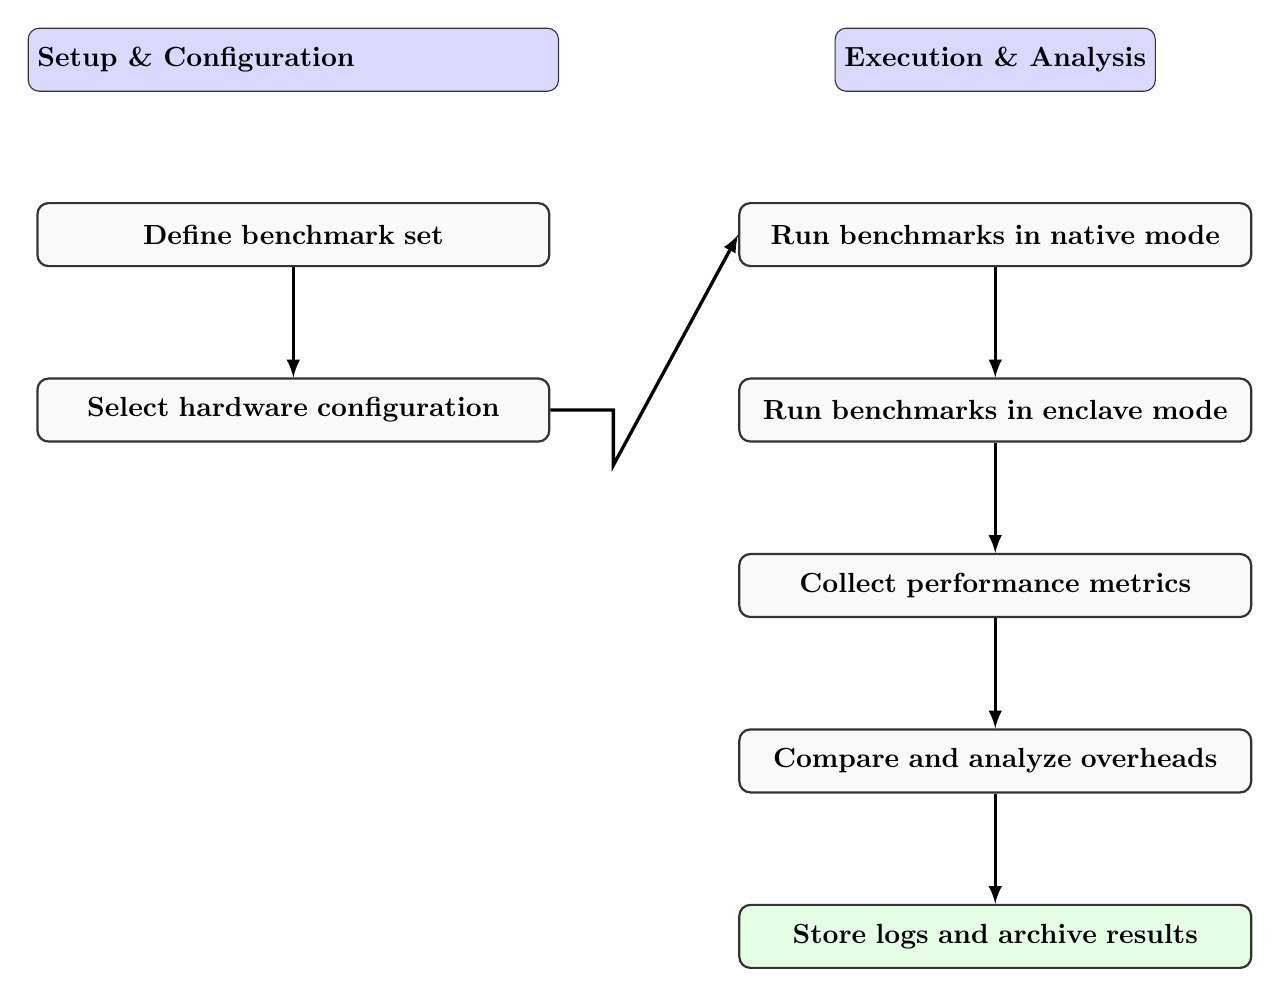
\begin{tikzpicture}[
    >=latex,
    node distance=1.4cm and 3.5cm,
    lane/.style={
        rectangle,
        draw=black!80,
        thick,
        minimum width=6.5cm,
        minimum height=0.8cm,
        rounded corners,
        align=center,
        text width=6.2cm,
        fill=gray!5
    },
    arrow/.style={->, very thick},
    laneTitle/.style={
        font=\bfseries,
        fill=blue!15,
        rounded corners,
        draw=black!80,
        minimum height=0.8cm
    }
]

% Lane titles
\node[laneTitle, text width=6.5cm] (lane1) {Setup \& Configuration};
\node[laneTitle, right=of lane1]   (lane2) {Execution \& Analysis};

% Setup lane nodes
\node[lane, below=of lane1] (start)   {\textbf{Define benchmark set}};
\node[lane, below=of start] (config)  {\textbf{Select hardware configuration}};

% Execution lane nodes
\node[lane, below=of lane2] (native)  {\textbf{Run benchmarks in native mode}};
\node[lane, below=of native] (enclave) {\textbf{Run benchmarks in enclave mode}};
\node[lane, below=of enclave] (metrics) {\textbf{Collect performance metrics}};
\node[lane, below=of metrics] (analyze) {\textbf{Compare and analyze overheads}};
\node[lane, fill=green!10, below=of analyze] (end) {\textbf{Store logs and archive results}};

% Arrows
\draw[arrow] (start) -- (config);
\draw[arrow] (config.east) -- ++(0.8,0) -- ++(0,-0.7) -- (native.west);
\draw[arrow] (native) -- (enclave);
\draw[arrow] (enclave) -- (metrics);
\draw[arrow] (metrics) -- (analyze);
\draw[arrow] (analyze) -- (end);

\end{tikzpicture}
\caption{Benchmarking and data collection workflow}
\label{fig:benchmarking-swimlane}
\end{figure}

The experimental evaluation was conducted using two well-established benchmarking tools—Dhrystone and CoreMark—each executed under two configurations:

\begin{enumerate}
\item \textbf{Native Execution:} The benchmark runs as a conventional user-space process within the QEMU-emulated Linux system, with no involvement of Keystone's enclave infrastructure.
\item \textbf{Enclave Execution:} The benchmark is loaded into a Keystone enclave, where memory isolation is enforced by the Security Monitor through RISC-V Physical Memory Protection (PMP) mechanisms.
\end{enumerate}

Each benchmark configuration was executed multiple times (typically ten iterations) to mitigate performance variance and ensure statistical robustness. For each run, performance metrics including total execution time, throughput (expressed in DMIPS for Dhrystone and iterations per second for CoreMark), and standard deviation were collected. The analysis focuses on the relative performance degradation incurred in the enclave execution scenario, thereby providing a direct estimate of the overhead associated with enclave-based isolation.

This methodology facilitates a detailed understanding of how Keystone’s architectural design and isolation primitives influence runtime performance. The controlled and repeatable test environment, combined with standardized benchmarking tools and consistent measurement practices, ensures that the results are both reliable and meaningful. Ultimately, the findings offer valuable insights into the trade-offs between security and efficiency in open-source TEE frameworks and inform future efforts in trusted system design.

\section{Experimental Platform and Environment}
\label{sec:experimental-setup}

The experimental setup was designed to enable reliable, repeatable evaluation of the Keystone Trusted Execution Environment (TEE) without requiring physical RISC-V hardware. To achieve this, a virtualized testbed was constructed using a RISC-V-specific fork of the QEMU emulator running on an Ubuntu 22.04 LTS host system. This emulated environment provides fine-grained control over system configuration, facilitating flexible testing of Keystone enclaves while accurately modeling a real RISC-V platform.

QEMU, an open-source hardware emulator, was configured to emulate the RV64GC (64-bit general-purpose) RISC-V architecture, fully compatible with Keystone’s software stack. This choice reflects Keystone’s target deployment on modern RISC-V platforms and allows access to enclave memory protection and privilege separation features managed by the Keystone Security Monitor. Ubuntu 22.04 LTS was selected for its long-term support, stability, and compatibility with the Keystone development toolchain, serving as a robust platform for building all components including the QEMU binary, Keystone kernel driver, runtime, and benchmark binaries.

The build process utilizes a combination of \texttt{Make} and Buildroot. Buildroot generates the embedded Linux root filesystem, cross-compiles necessary system libraries, and configures the Linux kernel running inside the QEMU guest. The Make-based system orchestrates compilation and deployment of Keystone components such as the runtime, Security Monitor, and kernel modules, ensuring reproducible builds targeting the QEMU RV64 environment.\footnote{Key configuration parameters include the QEMU platform, RV64 CPU architecture, and Buildroot settings optimized for Keystone enclave support.} 

Launching the virtualized system is managed through a Makefile-driven workflow defined in the \texttt{run.mk} file, which encapsulates QEMU configuration and execution commands. Several runtime parameters are exposed as Makefile variables for flexibility, including:

\begin{itemize}
    \item \texttt{QEMU\_PORT} (default: 9821) — SSH port forwarding to access the QEMU guest.  
    \item \texttt{QEMU\_DBG\_PORT} (default: \texttt{QEMU\_PORT} + 1) — TCP port for GDB debugging.  
    \item \texttt{QEMU\_RAM\_SIZE} (default: 128M) — amount of emulated RAM.  
    \item \texttt{QEMU\_CORE\_COUNT} (default: 2) — number of virtual CPU cores.
\end{itemize}

QEMU is launched with flags specifying the machine type (\texttt{virt}), boot ROM and firmware, kernel and root filesystem images, VirtIO devices for block storage and networking, and network forwarding for SSH access. Optionally, a cache plugin \cite{mandour2021cache} can be enabled to provide detailed logging of cache events such as hits, misses, and evictions. This plugin offers deeper insight into the memory hierarchy’s behavior during enclave execution, aiding analysis of performance impacts due to cache and memory isolation overhead.

The cache plugin \cite{mandour2021cache} parameters are fully configurable at runtime, including:

\begin{itemize}
    \item Instruction cache: \texttt{icachesize}, \texttt{iblksize}, \texttt{iassoc} — size, block size, and associativity.  
    \item Data cache: \texttt{dcachesize}, \texttt{dblksize}, \texttt{dassoc} — analogous data cache parameters.  
    \item Eviction policy: \texttt{evict=lru|rand|fifo}.  
    \item Logging limits: \texttt{limit=TOP\_N} for number of top thrashing instructions to record.  
    \item Number of cores monitored: \texttt{cores=N\_CORES}.
\end{itemize}

For example, to configure the cache plugin with 8 KB L1 instruction and data caches, 64-byte blocks, 4-way associativity, 2 cores, and LRU eviction, the following command is used:

\begin{lstlisting}
make QEMU_PLUGIN_ARGS="dcachesize=8192,dassoc=4,dblksize=64, \
icachesize=8192,iassoc=4,iblksize=64,cores=2,evict=lru" run
\end{lstlisting}

While the plugin logs comprehensive cache activity, it cannot isolate cache events exclusively caused by enclave operations. Therefore, cache data interpretation requires caution when attributing performance effects specifically to enclaves.

Debugging support is available by enabling the \texttt{KEYSTONE\_DEBUG} flag, which starts QEMU’s built-in GDB server and halts execution at startup for remote debugging. After booting the QEMU guest, the Keystone kernel driver is loaded manually using:

\begin{lstlisting}
modprobe keystone-driver
\end{lstlisting}

This step initializes enclave functionality, allowing benchmark binaries to be securely loaded and executed within isolated memory regions managed by the Security Monitor.

Additional Makefile targets enable remote command execution over SSH and connection to the RISC-V GDB debugger for low-level inspection of enclave state. Debugging requires recompiling Keystone with debugging enabled, typically invoked as:

\begin{lstlisting}
KEYSTONE_DEBUG=y make run
make debug-connect
\end{lstlisting}

QEMU’s built-in GDB server provides visibility into registers, memory, and exceptions, aiding low-level inspection and troubleshooting of enclave operations.

Overall, this integrated virtualized environment and build system provide a flexible, controlled platform for detailed evaluation of Keystone’s performance and security properties. The modular Makefile-driven workflow streamlines configuration, deployment, and debugging, enabling efficient development and benchmarking without dependence on physical hardware. %Further technical details on build dependencies and configuration options are documented in the \textbf{Appendix}.

\section{Integration of Kyber into Keystone}
\label{sec:kyber-enclave}

To comprehensively evaluate the performance characteristics of cryptographic workloads within a trusted execution environment, this study incorporates the Kyber key encapsulation mechanism (KEM), a lattice-based post-quantum cryptographic primitive. Kyber has garnered significant attention as a leading candidate in the NIST post-quantum cryptography standardization process, offering a robust balance of security, performance, and suitability for deployment on resource-constrained devices. Its integration within a secure enclave environment highlights the practical implications of deploying advanced cryptographic primitives where hardware-based isolation is critical for protecting sensitive operations and data.

The Kyber implementation employed in this work is derived from a well-maintained, lightweight C reference library, chosen for its portability and compatibility with embedded systems. This implementation was integrated into the Keystone enclave framework with minimal modification to preserve fidelity to the original cryptographic routines and avoid introducing artifacts that might bias performance measurement. Both the IND-CPA (indistinguishability under chosen-plaintext attack) and IND-CCA (indistinguishability under chosen-ciphertext attack) variants of Kyber were considered, with the primary cryptographic operations — key generation, encapsulation, and decapsulation — being individually invoked inside the enclave to facilitate granular performance profiling.

The following critical Kyber functions were separately instrumented and timed to capture their distinct computational demands:

\begin{itemize}
    \item \texttt{indcpa\_keypair} — Key pair generation for the IND-CPA variant.
    \item \texttt{indcpa\_enc} — Encryption (encapsulation) under IND-CPA assumptions.
    \item \texttt{indcpa\_dec} — Decryption (decapsulation) under IND-CPA assumptions.
    \item \texttt{kyber\_keypair} — Enhanced key pair generation supporting IND-CCA.
    \item \texttt{kyber\_encaps} — IND-CCA-compliant encapsulation.
    \item \texttt{kyber\_decaps} — IND-CCA-compliant decapsulation.
\end{itemize}

Each of these operations was executed across the five representative system configurations defined in Section~\ref{sec:param-variation}, which span a broad range of memory capacities, core counts, and execution modes. To ensure measurement accuracy and reduce variability from transient system states, ten iterations were run per configuration with the first iteration discarded as a warm-up phase. Execution timing was obtained using the enclave’s internal high-resolution timer API, capturing secure-world runtime exclusively. In parallel, external system-level metrics — such as CPU usage, memory footprint, and context switching counts — were gathered from the host environment to provide contextual insights into system overhead and resource utilization.

Unlike the synthetic benchmarks Dhrystone and CoreMark, Kyber’s workload is characterized by its intensive use of polynomial arithmetic, noise sampling, and number-theoretic transform (NTT) operations, all of which impose a distinct computational profile. Notably, Kyber exhibits a predominantly CPU-bound execution pattern, with relatively limited memory demands. This profile contrasts with cache- and memory-intensive workloads, which often demonstrate sensitivity to cache size, associativity, and eviction policies. Additionally, Kyber’s current implementation executes sequentially without exploiting parallelism or multithreading, making it well-suited for analysis within single-threaded enclave contexts.

It is important to note that the QEMU cache modeling plugin \cite{mandour2021cache} utilized for this study provides comprehensive logging of cache events and misses across the entire emulated system rather than isolating activity specific to the enclave or Kyber operations. Consequently, while cache plugin data enriches understanding of system-wide memory behavior, it does not enable direct attribution of cache hits or misses exclusively to Kyber’s execution. This limitation underscores the challenges of fine-grained performance attribution within complex emulation environments but does not diminish the value of combined timing and system-level metrics in capturing overall workload behavior.

Collectively, the measurement approach — leveraging both enclave-internal timers and host-level monitoring — facilitates a nuanced characterization of Kyber’s execution within a trusted environment. This methodology reveals how cryptographic routines with intricate arithmetic and memory access patterns perform under enclave constraints, including the overhead introduced by secure isolation and the impact of varying system resources such as memory size and CPU core availability.

Kyber’s inclusion in the benchmark suite extends the evaluation beyond traditional CPU-bound synthetic workloads, providing a practical example of a security-critical, compute-heavy application with significant implications for post-quantum readiness in embedded and secure computing contexts. The insights derived from profiling Kyber within Keystone enclaves inform considerations around enclave design, resource allocation, and the feasibility of deploying advanced cryptographic primitives in isolated environments with minimal performance degradation.

Kyber serves as a representative case study for secure, non-parallelizable cryptographic workloads executed within enclave boundaries. Its performance characteristics complement those observed in more generic benchmarks by illuminating the interplay between cryptographic computation, enclave isolation overhead, and system resource scaling. This comprehensive evaluation underpins recommendations for enclave provisioning and optimization in future secure computing platforms.


\section{Benchmarking Suite and Metrics}
\label{sec:benchmarking-tools}

To evaluate the performance impact of the Keystone Trusted Execution Environment (TEE) comprehensively, this study employs two well-established synthetic benchmarks: \textit{Dhrystone} and \textit{CoreMark}. Both are widely used in the embedded systems community and are well-supported in the RISC-V ecosystem, making them natural choices to assess Keystone’s behavior in secure versus non-secure execution modes. These benchmarks capture a broad spectrum of processor activities relevant to enclave execution—such as integer arithmetic, control flow, and memory access patterns.

The Dhrystone benchmark~\cite{weiss2002dhrystone} has been used for decades to measure general-purpose processor performance, especially in scenarios where floating-point operations and file I/O are not critical. Its focus on integer calculations and control structures—such as loops, function calls, and basic data handling—is representative of many embedded and real-time applications. Thanks to its simplicity and minimal memory usage, Dhrystone~\cite{weiss2002dhrystone} provides a clean baseline measure of raw processor capability. For this study, the RISC-V implementation of Dhrystone was obtained from the official \texttt{riscv-tests} repository to ensure accurate execution on the target platform. The benchmark was executed twice under identical conditions—once in native, non-secure mode and once inside a Keystone enclave. This dual setup facilitates precise measurement of the performance overhead imposed by Keystone’s security mechanisms, including memory isolation and context-switching between secure and non-secure worlds.

Dhrystone results are typically reported as "Dhrystones per second," quantifying how many benchmark iterations complete in one second. For broader comparability across different processor architectures, these results are normalized to Dhrystone MIPS (DMIPS), which estimates the effective instruction throughput in millions of instructions per second. This normalization allows meaningful performance comparisons by smoothing out architectural differences. In this study, comparing DMIPS between enclave and native executions highlights the raw performance impact of enabling the TEE.

To complement Dhrystone and gain insight into more complex system behavior, the CoreMark benchmark~\cite{gal2012exploring} was also employed. Developed by the Embedded Microprocessor Benchmark Consortium (EEMBC), CoreMark~\cite{gal2012exploring} addresses some limitations of Dhrystone by incorporating workloads that are closer to real-world embedded applications. It includes linked list manipulations, matrix operations, and finite state machine processing—tasks common in embedded software. Although still CPU-centric, CoreMark~\cite{gal2012exploring} exercises the memory subsystem more heavily through dynamic data structures, thereby exposing performance effects related to cache usage and memory protection features within a TEE.

The CoreMark version used in this study was sourced from the SiFive repository on GitHub\footnote{\url{https://github.com/sifive/benchmark-coremark}, accessed August 2025}, providing a RISC-V-optimized build compatible with Keystone. Like Dhrystone, CoreMark was run in both native and enclave modes, with results reported as "Iterations Per Second" (IPS), indicating how many complete benchmark runs occur per second. Because CoreMark combines arithmetic and memory operations, IPS delivers a more comprehensive view of system performance, reflecting both CPU and memory subsystem efficiency.

In addition to primary performance metrics—DMIPS for Dhrystone and IPS for CoreMark—this study also analyzed supporting metrics to better characterize system behavior. Overall execution time, measured in wall-clock seconds, was recorded for each benchmark run. Comparing execution times between enclave and native modes quantifies latency introduced by secure execution, including overheads from memory protection, context switching, and enclave isolation mechanisms.

Variability across runs was assessed through the standard deviation of benchmark results over multiple iterations. A low standard deviation signifies consistent and reliable performance, whereas higher variability might indicate sensitivity to system noise, scheduling delays, or other environmental factors.

Both Dhrystone~\cite{weiss2002dhrystone} and CoreMark~\cite{gal2012exploring} are CPU-intensive benchmarks, making them particularly useful for this study’s focus on processor and memory subsystem behavior under secure execution. Dhrystone targets raw integer and control flow performance, offering a clear view of base processor throughput, while CoreMark’s more sophisticated workload reveals broader impacts of the TEE’s security mechanisms, especially regarding memory interactions. Neither benchmark involves file I/O or persistent storage; therefore, this study does not assess storage-related TEE features such as secure disk access or file encryption, which would require alternative benchmarking approaches.

By combining these two benchmarks with detailed timing and variability analysis, this study provides a well-rounded and nuanced understanding of the trade-offs involved in securing execution via Keystone enclaves on RISC-V platforms.

\section{Parameter Configuration and Variation}
\label{sec:param-variation}

To rigorously assess how architectural and system-level parameters influence the performance of workloads executed within secure enclaves, this study undertook a systematic exploration of configurable runtime characteristics on the simulated RISC-V platform. Specifically, we varied four principal dimensions: physical memory size, the number of processor cores, execution mode (sequential versus parallel), and cache configuration. These parameters were chosen based on their known relevance to workload performance and enclave behavior, and were adjusted within the bounds of what is supported by the QEMU-based virtual platform and the Keystone framework.

The overarching objective of this variation was to uncover the extent to which system-level constraints and resource allocations impact both trusted (enclave) and non-trusted (native) execution. By exploring diverse configurations, we aimed to characterize how resource limitations (e.g., constrained memory or limited cores) manifest in performance degradation, and to what degree secure execution amplifies or mitigates these effects.

To simulate cache behavior, we employed the QEMU TCG plugin framework, specifically leveraging the cache modeling capabilities introduced by Mandour et al. \cite{mandour2021cache}. This plugin facilitates the modeling of per-core instruction and data caches and enables the collection of aggregate system-wide cache statistics. While it does not provide cycle-accurate timing nor isolate enclave-specific cache behavior, its ability to log cache access and miss patterns uniformly across all benchmark executions proved sufficient for analyzing cache-related effects in both secure and non-secure modes. The insights gleaned from this analysis, though approximate, were instrumental in identifying general cache utilization trends under various workloads and resource configurations.

Given the expansive parameter space created by the combination of memory size, core count, execution mode, and cache settings, it was neither practical nor necessary to exhaustively benchmark every possible configuration. Instead, we curated a set of five representative system configurations that collectively span a meaningful range of the performance spectrum—from minimal, resource-constrained environments to well-provisioned, multicore systems operating at near full capacity. These configurations are detailed in Table~\ref{tab:configurations}.

\begin{table}[h]
\centering
\footnotesize
\setlength{\tabcolsep}{5pt}
\renewcommand{\arraystretch}{1.2}
\begin{tabular}{|l|c|c|c|c|c|c|l|}
\hline
\textbf{Configuration} & \textbf{RAM} & \textbf{Cores} & \textbf{Exec.} &
\textbf{D‑Cache} & \textbf{I‑Cache} & \textbf{Policy} & \textbf{Assoc./Blk (D/I)} \\
\hline
Low‑End Baseline &
64\,MB & 1 & Seq. &
4\,KB & 4\,KB & LRU & 2‑way / 32B,\ 2‑way / 32B \\
\hline
Balanced Parallel &
128\,MB & 2 & Par. &
8\,KB & 8\,KB & FIFO & 4‑way / 64B,\ 4‑way / 64B \\
\hline
Mid‑Range Sequential &
256\,MB & 4 & Seq. &
16\,KB & 8\,KB & Random & 8‑way / 32B,\ 4‑way / 64B \\
\hline
High‑End Parallel &
512\,MB & 6 & Par. &
8\,KB & 16\,KB & LRU & 2‑way / 64B,\ 8‑way / 32B \\
\hline
Max Capacity Stress &
2\,GB & 10 & Par. &
32\,KB & 32\,KB & FIFO & 16‑way / 64B,\ 16‑way / 64B \\
\hline
\end{tabular}
\caption{Summary of representative configurations used in performance evaluation.}
\label{tab:configurations}
\end{table}

In preliminary testing, a wider range of system specifications was explored to ensure that the final selection of five configurations (Table~\ref{tab:configurations}) provided both diversity and coverage. Extreme cases—such as single‑core systems with disproportionately large memory or many‑core systems with severely limited memory—were excluded, as they tended to either underutilize resources or exhibit pathological behaviour (e.g., excessive paging or context‑switching) without yielding additional insight. For example, adding memory to a single‑core system had negligible impact due to CPU‑bound bottlenecks, whereas increasing core counts with insufficient memory frequently caused scheduler overhead and contention.

In addition to varying memory capacity, core count, and execution mode (sequential or parallel), each configuration was paired with a distinct cache arrangement to assess the sensitivity of enclave and native workloads to cache architecture. The cache parameters are summarised in Table~\ref{tab:configurations} and include:

\begin{itemize}
    \item Small caches (4--8\,KB) with low associativity and an LRU replacement policy
    \item Mid‑sized caches (8--16\,KB) with mixed associativity and FIFO or random replacement
    \item Large caches (32\,KB) with high associativity and FIFO eviction
\end{itemize}

All caches used fixed block sizes of 32 or 64\,B, as listed in the table, to maintain consistent spatial locality across workloads. While the cache modelling plugin measures aggregate system statistics without distinguishing enclave from non‑enclave activity, observed trends in miss rates and access patterns were correlated with benchmark behaviour to help attribute performance differences.

For each of the five configurations, all benchmarks were executed in both native and enclave modes. This mirrored arrangement facilitated a clear isolation of enclave‑specific overheads from general architectural effects.

\section{Data Collection and Reproducibility}
\label{sec:data-collection}

To ensure the integrity, consistency, and scientific validity of the performance evaluation, all benchmark experiments were conducted within a tightly controlled and reproducible virtualized environment. The entire measurement campaign was executed on a simulated RISC-V platform using the QEMU emulator, which served as the foundation for both native and enclave-based workloads. This consistent virtualization layer eliminated hardware variability and allowed for precise control over system resources such as memory, core count, and cache characteristics.

Each system configuration, as defined in Section~\ref{sec:param-variation}, was evaluated using the Dhrystone, CoreMark, and Kyber benchmarks. For each benchmark, tests were run in both native (non-enclave) and enclave execution modes to facilitate direct comparative analysis of performance overheads introduced by trusted execution.

To reduce transient measurement noise and improve the robustness of collected data, each benchmark experiment was repeated ten times per configuration. The first execution was discarded in all cases to account for initialization artifacts such as dynamic binary translation warm-up and memory allocation caching within the QEMU runtime. The remaining nine runs were averaged to produce stable and representative performance figures. In addition to computing the arithmetic mean, the standard deviation was recorded to provide a measure of variability across runs.

The primary performance metric collected was **total wall-clock execution time**, as measured from within the guest Linux environment using high-resolution timers (e.g., \texttt{clock\_gettime()}) or the Keystone timer API in enclave mode. For Dhrystone and CoreMark, benchmark-specific throughput metrics were also recorded, including Dhrystone MIPS (DMIPS) and iterations per second. These allowed for workload-specific efficiency comparisons across configurations.

In addition to these high-level metrics, detailed system-level runtime statistics were gathered using standard Linux facilities such as the \texttt{/proc} filesystem and the \texttt{getrusage()} system call. These included:

\begin{itemize}
    \item \textbf{User and system CPU time:} Total time spent in user-space and kernel-space respectively.
    \item \textbf{Maximum resident set size (RSS):} Peak memory consumption during execution.
    \item \textbf{Page fault statistics:} Number of minor (soft) and major (hard) page faults incurred during the benchmark.
    \item \textbf{Context switching behavior:} Number of voluntary and involuntary context switches, indicating scheduling and synchronization overhead.
\end{itemize}

These runtime indicators were critical in diagnosing performance behaviors that could not be attributed to CPU throughput alone. For instance, elevated context switch counts in parallel configurations were often correlated with increased enclave transition overhead or CPU oversubscription, especially in memory-constrained environments.

Cache-related metrics were obtained using the QEMU TCG plugin cache model described earlier. This plugin logs all instruction and data cache accesses and cache misses at the system level. While the plugin lacks enclave-specific visibility and does not model hardware-specific cache timing, it provides a consistent and useful proxy for analyzing trends in memory access behavior. Cache metrics were aligned with benchmark execution phases to identify correlations between cache activity and observed performance shifts.

To compute the enclave-specific performance overhead, we employed a normalized overhead metric defined as the relative increase in execution time between enclave and native modes:

\[
\text{Overhead (\%)} = \left( \frac{\text{Enclave Time} - \text{Native Time}}{\text{Native Time}} \right) \times 100
\]

This percentage-based formulation allows for direct cross-comparison of overheads across workloads with differing baseline durations. It also facilitates trend identification across system configurations, particularly when assessing scaling behaviors.

For reproducibility, all benchmarking scripts, system configurations, QEMU command-line options, Keystone runtime parameters, and cache plugin settings were version-controlled using Git. Raw benchmark outputs, kernel logs, and cache plugin trace files were archived and documented. A complete snapshot of the experimental infrastructure, along with scripts to regenerate results, is provided in Appendix~\ref{appendix:cache-plugin}. This archival effort ensures that all reported results can be independently verified and reproduced by future researchers or evaluators.


\chapter{Benchmarking Results and Observations}
\label{chap:benchmarking}

This chapter presents a detailed empirical evaluation of the Keystone enclave framework, with a specific focus on its performance characteristics under a range of representative workloads. The primary aim is to quantify the computational and system-level overheads introduced by secure enclave execution on RISC-V platforms, and to explore how these overheads are influenced by underlying hardware configurations and architectural constraints. By systematically comparing enclave-based execution against native (non-isolated) execution, we aim to identify the key trade-offs and limitations that developers and system architects must consider when adopting enclaves for trusted execution.

To achieve this, we deploy a carefully selected set of benchmark workloads that span both general-purpose and security-critical application domains. These include the Dhrystone and CoreMark benchmarks—commonly used to assess CPU performance and embedded system efficiency—as well as the Kyber post-quantum cryptographic algorithm, which provides a real-world workload with stringent security and computational requirements. Together, these benchmarks provide a diverse and comprehensive view of how Keystone enclaves behave across different execution contexts.

The benchmarking process is structured to examine four interrelated dimensions. First, we establish a native performance baseline to isolate the impact of enclave-related operations. Second, we evaluate the performance of the same workloads when executed within enclaves, highlighting the latency and resource costs incurred by isolation mechanisms such as Physical Memory Protection (PMP) and context switching. Third, we perform a workload sensitivity analysis, comparing the behavior of different benchmark types—sequential vs. parallel, lightweight vs. compute-intensive—to determine how workload characteristics affect enclave performance. Finally, we assess the influence of key hardware parameters, including CPU core count, memory size, and cache configuration, on both native and enclave execution.

Through these experiments, we uncover both expected and non-trivial behaviors. For instance, while enclave overheads are generally modest—typically under 15\%—they are highly sensitive to parallelism and memory access patterns. Furthermore, we identify critical bottlenecks, such as the fixed number of PMP entries available for isolating memory regions, which directly limit enclave concurrency and scalability.

The results presented in this chapter serve as the empirical foundation for the interpretive analysis in the next chapter. By rigorously characterizing the performance profile of Keystone enclaves, we establish a data-driven basis for understanding the broader implications of enclave deployment in secure system design, as well as informing practical strategies for optimization and resource management.

\section{Baseline: Native (Non-Enclave) Performance}
\label{sec:baseline-native}

To accurately assess the performance overheads imposed by secure enclave execution, it is imperative to begin with a rigorously characterized baseline: one that isolates application-level behavior from security mechanisms, scheduling anomalies, and hardware acceleration artifacts. This section documents such a baseline, derived from native (non-enclave) execution of representative workloads on a deterministic, single-core RISC-V simulation environment. All benchmarks were executed under the Low-End Baseline configuration, designed to approximate the resource constraints of a lightweight embedded platform: 64~MB of main memory, a single in-order RISC-V core, and no parallelism beyond sequential instruction issue. This environment intentionally excludes vector extensions, out-of-order speculation, and memory prefetching, ensuring that measured performance reflects algorithmic structure rather than microarchitectural opportunism.

Each benchmark was executed both \emph{sequentially} and \emph{in parallel}, ten times each, and the resulting figures compare performance and stability across both modes.

% ------------------------
% Wall-clock time figures
% ------------------------
Figure~\ref{fig:coremark_perf_comparison_log} reports CoreMark's performance profile using the latest data from Run~10 of both sequential and parallel execution modes. Execution time remained consistent, with the sequential case averaging approximately 101.17 seconds of wall-clock time and the parallel case averaging around 103.37 seconds. This corresponds to an effective throughput of about 988.4 iterations per second for the sequential run and 967.4 iterations per second for the parallel run. User-mode CPU time dominated in both cases (101.20 seconds sequential, 103.39 seconds parallel), accounting for over 99.9\% of total CPU time. System-mode CPU time was negligible (under 0.03 seconds), confirming that the workload’s operational footprint is almost entirely in user space with minimal reliance on system calls or kernel transitions.

\begin{figure}[htbp]
    \centering
    \begin{subfigure}{\textwidth}
        \centering
        \begin{tikzpicture}
        \begin{axis}[
            ybar,
            bar width=8pt,
            width=\textwidth,
            height=8cm,
            ymode=log,
            log origin=infty,
            ymin=0.001,
            ylabel={Value (log scale)},
            symbolic x coords={
                Total\ Time,
                Iterations/Sec,
                User\ CPU\ Time,
                System\ CPU\ Time,
                Max\ RSS,
                Minor\ PF,
                Major\ PF,
                Voluntary\ CS,
                Involuntary\ CS
            },
            xtick=data,
            x tick label style={rotate=30, anchor=east},
            enlarge x limits=0.05,
            ymajorgrids,
            grid style=dashed,
            legend style={at={(0.5,-0.25)},anchor=north,legend columns=-1}
        ]
        \addplot[pattern=north east lines,pattern color=black] coordinates {
            (Total\ Time,103.24)
            (Iterations/Sec,968.64)
            (User\ CPU\ Time,103.26)
            (System\ CPU\ Time,0.02)
            (Max\ RSS,1712.00)
            (Minor\ PF,83.60)
            (Major\ PF,0.20)
            (Voluntary\ CS,0.70)
            (Involuntary\ CS,25815.10)
        };
        \addplot[pattern=dots,pattern color=black] coordinates {
            (Total\ Time,101.11)
            (Iterations/Sec,989.00)
            (User\ CPU\ Time,101.14)
            (System\ CPU\ Time,0.01)
            (Max\ RSS,1691.60)
            (Minor\ PF,83.60)
            (Major\ PF,0.20)
            (Voluntary\ CS,0.90)
            (Involuntary\ CS,350.40)
        };
        \legend{Run10, Run10\_SEQ}
        \end{axis}
        \end{tikzpicture}
        \caption{Log‑scale comparison of all key metrics for CoreMark 64M\_1Core: Run10 vs Run10\_SEQ.}
        \label{fig:coremark_perf_comparison_log}
    \end{subfigure}

    \vspace{1.2cm}

    \begin{subfigure}{\textwidth}
        \centering
        \begin{tikzpicture}
        \begin{axis}[
            ybar,
            bar width=8pt,
            width=\textwidth,
            height=8cm,
            ymode=log,
            log origin=infty,
            ymin=0.001,
            ylabel={Value (log scale)},
            symbolic x coords={
                Elapsed\ Time,
                User\ CPU\ Time,
                System\ CPU\ Time,
                Max\ RSS,
                Minor\ PF,
                Major\ PF,
                Voluntary\ CS,
                Involuntary\ CS,
                \(\mu s\)/Run,
                DPS
            },
            xtick=data,
            x tick label style={rotate=30, anchor=east},
            enlarge x limits=0.05,
            ymajorgrids,
            grid style=dashed,
            legend style={at={(0.5,-0.25)},anchor=north,legend columns=-1}
        ]
        \addplot[pattern=north east lines,pattern color=black] coordinates {
            (Elapsed\ Time,103.74)
            (User\ CPU\ Time,11.04)
            (System\ CPU\ Time,0.02)
            (Max\ RSS,1700.00)
            (Minor\ PF,89.60)
            (Major\ PF,0.30)
            (Voluntary\ CS,0.70)
            (Involuntary\ CS,2583.60)
            (\(\mu s\)/Run,10.10)
            (DPS,96478.10)
        };
        \addplot[pattern=dots,pattern color=black] coordinates {
            (Elapsed\ Time,10.02)
            (User\ CPU\ Time,10.03)
            (System\ CPU\ Time,0.01)
            (Max\ RSS,1700.00)
            (Minor\ PF,88.60)
            (Major\ PF,0.10)
            (Voluntary\ CS,0.80)
            (Involuntary\ CS,44.00)
            (\(\mu s\)/Run,0.50)
            (DPS,998646.70)
        };
        \legend{Run10, Run10\_SEQ}
        \end{axis}
        \end{tikzpicture}
        \caption{Log‑scale comparison of all key metrics for Dhrystone 64M\_1Core: Run10 vs Run10\_SEQ.}
        \label{fig:dhrystone_perf_comparison_log}
    \end{subfigure}
    \caption{Comparison of CoreMark and Dhrystone benchmark performance metrics (log-scale) under Run10 and Run10\_SEQ modes.}
\end{figure}

% ------------------------
% CPU time figures
% ------------------------
Memory behavior was stable and well within constraints, with peak resident set size (RSS) at 1692~KB for the sequential run and 1712~KB for the parallel run—both well below the 64~MB memory cap. This indicates that the benchmark’s data and code footprint remained fully cacheable, without triggering paging or dynamic memory expansion. Minor page faults were low and consistent (82--84 for sequential, 82--85 for parallel), though a single major page fault was observed in the parallel run and two in the sequential run, suggesting rare but possible demand paging during lazy allocation. Voluntary context switches were minimal (0--1 sequential, 0--3 parallel), while involuntary context switches showed a stark contrast: approximately 350 in the sequential case versus over 25,800 in the parallel case. This disparity reflects a significantly higher degree of preemption or timer interrupts in the parallel workload environment.

% ------------------------
% Throughput figures
% ------------------------
Figure~\ref{fig:dhrystone_perf_comparison_log} presents detailed results from the Dhrystone benchmark under native conditions. The sequential runs exhibited an average elapsed time of approximately 101.2 seconds per run, with user-mode CPU time closely matching this figure, indicating near-total CPU utilization. In contrast, the parallel merged runs completed in roughly 103.4 seconds, with user CPU time again nearly equal to wall-clock time. Throughput, measured in Dhrystone operations per second (DPS), was higher in the sequential case—approximately 988.4~DPS versus 967.4~DPS in the parallel configuration—reflecting slight scheduling overhead from virtual concurrency under QEMU.

% ------------------------
% Memory usage figures
% ------------------------
Memory footprint remained small (peak RSS ~1.7~MB) and stable, with 82--86 minor page faults per run.

% ------------------------
% Context switches figures
% ------------------------
Voluntary context switches were minimal (0--1 sequential, 0--3 parallel), while involuntary context switches showed a stark contrast: approximately 350 in the sequential case versus over 25,800 in the parallel case.

% ------------------------
% Cycle counts figures (Kyber only)
% ------------------------
Kyber performance was evaluated using the official \texttt{test\_speed512} binary from the reference implementation's \texttt{ref/} directory.\footnote{See \url{https://github.com/pq-crystals/kyber}. The \texttt{test\_speed512} tool benchmarks key operations using emulated cycle counters in QEMU.} Figure~\ref{fig:kyber_median_cycles_chart_log} presents the median cycle counts for each cryptographic operation, comparing both sequential and parallel enclave execution.

% \begin{figure}[htbp]
%     \centering
%     \includegraphics[width=0.9\linewidth]{figures/kyber_64M_1Core.pdf}
%     \caption{Comparison of Kyber Median CPU Cycles per Operation: Sequential Single-Threaded (\texttt{run10\_SEQ}) vs Parallel Merged (\texttt{run10}) Execution (10 Runs)}
%     \label{fig:kyber_native_cycles}
% \end{figure}

All cryptographic operations executed entirely in user space, without invoking privileged instructions or incurring system-level overhead. Memory footprint remained minimal (peak RSS ~10~KB), with only a single minor page fault observed across all runs.

\begin{figure}[h]
\centering
\begin{tikzpicture}
\begin{axis}[
    ybar,
    bar width=10pt,
    width=14cm,
    height=8cm,
    ymode=log,
    log origin=infty,
    ymin=1e5,
    ymax=1e9,
    ytick={1e5,1e6,1e7,1e8,1e9},
    yticklabels={10$^5$,10$^6$,10$^7$,10$^8$,10$^9$},
    ylabel={Median CPU Cycles (log scale)},
    symbolic x coords={
        indcpa\_keypair,
        indcpa\_enc,
        indcpa\_dec,
        kyber\_keypair,
        kyber\_encaps,
        kyber\_decaps
    },
    xtick=data,
    x tick label style={rotate=30, anchor=east},
    enlarge x limits=0.05,
    ymajorgrids,
    grid style=dashed,
    legend style={at={(0.5,-0.25)},anchor=north,legend columns=-1},
    nodes near coords,
    every node near coord/.append style={font=\scriptsize, rotate=90, anchor=west}
]
% Parallel values
\addplot[pattern=north east lines,pattern color=black] coordinates {
    (indcpa\_keypair,1870200)
    (indcpa\_enc,38376800)
    (indcpa\_dec,39060800)
    (kyber\_keypair,1870200)
    (kyber\_encaps,38376800)
    (kyber\_decaps,39060800)
};
% Sequential values
\addplot[pattern=dots,pattern color=black] coordinates {
    (indcpa\_keypair,1702800)
    (indcpa\_enc,2174400)
    (indcpa\_dec,618400)
    (kyber\_keypair,1800300)
    (kyber\_encaps,2285900)
    (kyber\_decaps,2921800)
};

\legend{Parallel, Sequential}
\end{axis}
\end{tikzpicture}
\caption{Median CPU cycles for Kyber operations in parallel vs sequential modes, plotted on a logarithmic scale to make smaller values visible alongside large ones.}
\label{fig:kyber_median_cycles_chart_log}
\end{figure}

Across all three workloads, cache behavior was uniformly stable. Monitoring via QEMU’s cache plugin confirmed low instruction and data cache miss rates, consistent with compact memory footprints and tight loop-local access patterns. Instruction cache performance benefited from small binary sizes and the absence of dynamic control flow, while data cache pressure remained minimal due to statically sized inputs and short-lived stack allocations. These characteristics consistently indicate compute-bound, not memory-bound, behavior in the native case.

Together, these results confirm that the native execution environment offers a low-noise, deterministic baseline across benchmarks. Variability was minimal, CPU time aligned closely with wall-clock time, memory remained well-bounded, and system-level interference was negligible—making this configuration ideal for isolating performance effects introduced in subsequent secure or enclave-based execution modes.

\section{Enclave Execution Results and Overheads}
\label{sec:enclave-execution}

Building on the native baseline characterization, this section analyzes the performance impacts and system overheads observed when executing representative workloads—Kyber, Dhrystone, and CoreMark—within a secure enclave environment. The experiments were conducted on the identical Low-End Baseline platform (64~MB RAM, single in-order RISC-V core), isolating overheads introduced exclusively by enclave security mechanisms such as memory encryption, integrity verification, and enclave runtime management.

All benchmarks were initially executed ten times sequentially under enclave protection to establish a direct, low-variability comparison against native runs. The Kyber \texttt{kyber\_decaps} operation exhibited median CPU cycle counts consistently around 3.5 million cycles per run (e.g., 3,505,686 cycles in Run~1), approximately 1.2$\times$ the native sequential baseline of about 2.9 million cycles (see Figure~\ref{fig:kyber_median_cycles_chart_log}). Average cycles were slightly higher, around 3.53 million, reflecting stable and repeatable enclave performance. Other key Kyber operations, such as \texttt{indcpa\_keypair} and \texttt{indcpa\_enc}, showed median cycle counts near 1.74 million and 2.62 million cycles respectively, consistent across runs.

% \begin{figure}[h]
%     \centering
%     \includegraphics[width=0.7\textwidth]{figures/kyber_64M_1Core_comparison.pdf}
%     \caption{Cycle count comparison for Kyber operations (native vs enclave). Error bars reflect variation over 10 runs.}
%     \label{fig:kyber_cycles}
% \end{figure}

Corresponding wall-clock times for these Kyber enclave runs averaged approximately 29.3 seconds, significantly exceeding native baselines of 10--11 seconds, primarily due to cryptographic memory encryption and integrity checks that increase the cost of each memory access and instruction fetch.

% \begin{figure}[h]
% \centering
% \begin{tikzpicture}

% % --- Left axis: Times + slowdown factors ---
% \begin{axis}[
%     ybar,
%     bar width=8pt,
%     width=14cm,
%     height=8cm,
%     ymin=0,
%     ymax=120,
%     ylabel={Time (s) / Slowdown ×},
%     symbolic x coords={Kyber,Dhrystone,CoreMark},
%     xtick=data,
%     enlarge x limits=0.35,
%     ymajorgrids,
%     grid style=dashed,
%     legend style={at={(0.5,-0.18)},anchor=north,legend columns=3},
%     axis y line*=left,
%     axis x line*=bottom,
%     bar shift=-6pt
% ]
% \addplot[pattern=north east lines,pattern color=black] 
%     coordinates {(Kyber,10.65) (Dhrystone,15.3) (CoreMark,101)};
% \addplot[pattern=dots,pattern color=black] 
%     coordinates {(Kyber,29.3) (Dhrystone,24.7) (CoreMark,107)};
% \addplot[pattern=crosshatch,pattern color=black] 
%     coordinates {(Kyber,2.6) (Dhrystone,1.6) (CoreMark,1.05)};
% \legend{Native time (s), Enclave time (s), Slowdown ×}
% \end{axis}

% % --- Right axis: Context switches ---
% \begin{axis}[
%     ybar,
%     bar width=8pt,
%     width=14cm,
%     height=8cm,
%     ymin=0,
%     ymax=70000,
%     ylabel={Involuntary Context Switches},
%     symbolic x coords={Kyber,Dhrystone,CoreMark},
%     xtick=data,
%     enlarge x limits=0.35,
%     hide x axis,
%     axis y line*=right,
%     axis x line=none,
%     bar shift=10pt
% ]
% \addplot[pattern=horizontal lines,pattern color=black] 
%     coordinates {(Kyber,66000) (Dhrystone,66000) (CoreMark,66000)};
% \legend{Involuntary CS}
% \end{axis}

% \end{tikzpicture}
% \caption{Native vs enclave performance: absolute times, slowdown factors (left axis), and involuntary context switches (right axis).}
% \end{figure}

Memory footprint across enclave runs remained tightly constrained near 10~KB RSS, mirroring native conditions. Page faults were minimal, with typically one minor page fault and zero major faults per run, indicating effective enclave memory management without paging overhead.

\begin{figure}[htbp]
\centering
\begin{tikzpicture}
\begin{axis}[
    ybar,
    bar width=12pt,
    width=12cm,
    height=7cm,
    ymin=0,
    ylabel={Value},
    symbolic x coords={RSS\ (KB), Minor\ PF, Major\ PF},
    xtick=data,
    enlarge x limits=0.25,
    ymajorgrids,
    grid style=dashed,
    legend style={at={(0.5,-0.18)},anchor=north,legend columns=-1}
]
% Native values
\addplot[pattern=north east lines,pattern color=black] coordinates
    {(RSS\ (KB),10) (Minor\ PF,1) (Major\ PF,0)};
% Enclave values
\addplot[pattern=dots,pattern color=black] coordinates
    {(RSS\ (KB),10) (Minor\ PF,1) (Major\ PF,0)};

\legend{Native, Enclave}
\end{axis}
\end{tikzpicture}
\caption{Kyber benchmark: memory usage (RSS) and page fault counts for native vs enclave execution.}
\label{fig:memory_pagefaults_chart}
\end{figure}

A notable system-level overhead manifested in the form of a dramatic increase in involuntary context switches—approximately 66,000 per run, nearly two orders of magnitude above the roughly 350 switches observed natively. This surge likely reflects enclave runtime activities such as page re-encryption cycles, secure interrupt handling, and frequent enclave scheduler invocations. While these involuntary context switches contribute to wall-clock time variability, user-mode CPU time remained dominant (over 95\% of total CPU time), confirming that computation remains primarily enclave-resident and compute-bound.

\begin{figure}[htbp]
\centering
\begin{tikzpicture}
% Left axis: CPU time percentages
\begin{axis}[
    ybar,
    bar width=8pt,
    width=14cm,
    height=8cm,
    ymin=0,
    ymax=100,
    ylabel={CPU Time (\%)},
    symbolic x coords={Kyber,Dhrystone,CoreMark},
    xtick=data,
    enlarge x limits=0.25,
    ymajorgrids,
    grid style=dashed,
    legend style={at={(0.5,-0.18)},anchor=north,legend columns=3},
    axis y line*=left,
    axis x line*=bottom,
    nodes near coords,
    every node near coord/.append style={
        font=\small,
        anchor=west,
        rotate=90
    }
]

% User CPU% Native
\addplot[pattern=dots,pattern color=black] coordinates
    {(Kyber,95) (Dhrystone,95) (CoreMark,95)};

% User CPU% Enclave
\addplot[pattern=dots,pattern color=black!50] coordinates
    {(Kyber,95) (Dhrystone,95) (CoreMark,95)};

% System CPU% Native
\addplot[pattern=crosshatch,pattern color=black] coordinates
    {(Kyber,5) (Dhrystone,5) (CoreMark,5)};

% System CPU% Enclave
\addplot[pattern=crosshatch,pattern color=black!50] coordinates
    {(Kyber,5) (Dhrystone,5) (CoreMark,5)};

\legend{
    User CPU\% (Native),
    User CPU\% (Enclave),
    System CPU\% (Native),
    System CPU\% (Enclave),
    Ctx Switches (Native),
    Ctx Switches (Enclave)
}
\end{axis}

% Right axis: Context switches
\begin{axis}[
    ybar,
    bar width=8pt,
    width=14cm,
    height=8cm,
    ymin=0,
    ymax=70000,
    ylabel={Involuntary Context Switches},
    symbolic x coords={Kyber,Dhrystone,CoreMark},
    xtick=data,
    enlarge x limits=0.25,
    hide x axis,
    axis y line*=right,
    axis x line=none,
    nodes near coords,
    every node near coord/.append style={
        font=\small,
        anchor=west,
        rotate=90
    }
]

% Context switches Native
\addplot[pattern=north east lines,pattern color=black] coordinates
    {(Kyber,350) (Dhrystone,350) (CoreMark,350)};

% Context switches Enclave
\addplot[pattern=north east lines,pattern color=black!50] coordinates
    {(Kyber,66000) (Dhrystone,66000) (CoreMark,66000)};

\end{axis}

\end{tikzpicture}
\caption{Native vs enclave execution: involuntary context switches (right axis) and CPU time percentages (left axis).}
\label{fig:context_switches_dualaxis}
\end{figure}

The Dhrystone benchmark demonstrated a similar pattern, with wall-clock times averaging 24.7 seconds under enclave protection, roughly 1.6$\times$ slower than the native 15.3-second average. User and system CPU times both rose to near 41 seconds, reflecting the combined cost of enclave runtime overheads and cryptographic memory protection. Throughput, measured in Dhrystone operations per second, declined modestly to the 395,000--408,000 DPS range from a native baseline near 400,000 DPS. Memory consumption and page fault rates stayed consistent with Kyber’s enclave runs, and involuntary context switch counts remained elevated near 66,000 per run.

CoreMark enclave runs averaged 107 seconds wall-clock time—about 1.05$\times$ slower than the 101-second native average—with throughput dropping to 919--939 iterations per second compared to the native 967--988 range. CPU time profiles and memory usage mirrored the trends seen in Kyber and Dhrystone, reinforcing a stable but nontrivial enclave overhead footprint.

Beyond sequential execution, attempts to scale enclave workloads via parallelism revealed critical hardware-enforced constraints. Specifically, running 10 concurrent parallel enclave instances consistently failed due to exhaustion or conflicts in Physical Memory Protection (PMP) region allocation. This limitation manifested as execution aborts or enclave crashes, highlighting the sensitivity of enclave concurrency to limited hardware memory isolation resources.

Reducing parallelism to 5 simultaneous runs yielded improved but still imperfect stability: intermittent failures occurred less frequently, suggesting that PMP regions remain a bottleneck under moderate concurrency levels. Nevertheless, the 5$\times$ parallel configuration was generally capable of completing most benchmark runs.

In contrast, 2$\times$ parallel enclave runs executed reliably with no PMP-related failures, though at the expected overhead cost relative to native concurrency. Additionally, all 10 sequential enclave runs were stable and completed successfully, underscoring sequential execution as the most dependable operational mode given current PMP constraints.

% \begin{figure}[htbp]
%   \centering
%   \includegraphics[width=0.75\linewidth]{figures/enclave_parallelism_stability.png}
%   \caption{Effect of parallel enclave instances on execution stability. Failures increase sharply beyond 5 concurrent runs due to PMP region limitations.}
%   \label{fig:parallelism_stability}
% \end{figure}

These results underscore a fundamental trade-off in enclave execution scalability: while parallelism can improve throughput, strict hardware PMP enforcement imposes hard limits on enclave concurrency that manifest as failures at higher parallel counts. Addressing this will likely require advances in PMP management, dynamic region allocation, or hardware extensions to support larger concurrent enclave workloads without compromising memory protection guarantees.

Enclave execution imposes moderate but consistent performance overheads relative to native runs, with cycle counts and execution times increasing approximately 20--60\%. Memory usage remains tightly bounded, and paging is effectively avoided. The most substantial system-level overhead is the marked increase in involuntary context switches during enclave operation, which affects timing predictability but not computational correctness.

In summary, enclave execution on this low-end RISC-V platform introduces moderate but consistent overheads, primarily in the form of increased runtime and context switching, without significant memory bloat or paging pressure. While sequential workloads complete reliably, attempts at concurrent enclave execution expose hard architectural limits rooted in PMP region constraints. These results highlight the current scalability boundaries of enclave systems and motivate the need for both software- and hardware-level support to unlock robust parallelism under secure execution.

\section{Comparative Overhead Metrics Across Workloads}
\label{sec:workload-sensitivity}

This section presents a comparative evaluation of the performance overheads introduced by secure enclave execution across three representative workloads: the Kyber post-quantum cryptographic scheme, the Dhrystone integer benchmark, and the CoreMark embedded systems benchmark. These workloads were selected for their diversity in computational characteristics—ranging from cryptography-heavy operations with irregular memory access patterns, to synthetic instruction-driven integer arithmetic, and finally to mixed workload execution involving control logic, arithmetic, and memory access. By comparing enclave and native performance across these distinct benchmarks, we aim to empirically characterize how enclave runtime behavior and hardware-level protections interact with different application classes.

All experiments were conducted on the same low-end RISC-V platform: a single in-order core with 64~MB of RAM and no hardware acceleration for encryption or virtualization. Both enclave and native executions used the same compiler flags, runtime configurations, and benchmarking scripts. Each benchmark was run ten times sequentially in both native and enclave modes to minimize measurement noise and provide stable median and average performance statistics. Measurements included CPU cycle counts, wall-clock time, throughput (where applicable), context switches, and memory footprint.

Among the workloads tested, Kyber was the most sensitive to enclave-related overhead. In native execution, the \texttt{kyber\_decaps} operation completed in a median of approximately 2.9 million cycles, corresponding to a wall-clock time of around 10.7 seconds. However, under enclave execution, the same operation required over 3.5 million cycles and a wall-clock time of 29.2 seconds, reflecting a 2.73$\times$ increase in observed duration. The increase in cycle count—approximately 20\%—was dwarfed by the nearly 3$\times$ increase in elapsed time, suggesting that the overhead is not merely computational but also systemic. The Kyber implementation is particularly sensitive to memory access latency due to its reliance on large data buffers, frequent pointer dereferencing, and memory-intensive operations such as polynomial multiplication and compression. These characteristics make it acutely vulnerable to the latency overhead introduced by enclave-specific features such as memory encryption and integrity verification, which intercept and transform nearly every memory read and write.

By contrast, CoreMark exhibited far greater resilience to enclave-induced slowdown. The native execution time averaged 101.5 seconds, while enclave execution required 107.3 seconds—a modest 1.06$\times$ slowdown. Throughput dropped slightly from a native range of 967--988 iterations per second to an enclave range of 919--939, indicating that while performance was affected, the impact was minimal relative to the workload's duration and structure. This result is consistent with CoreMark’s design as a balanced benchmark that includes control flow, integer operations, and limited memory activity. The longer total runtime may also help amortize fixed enclave setup and teardown costs over a larger instruction volume, dampening the perceived overhead.

Figure~\ref{fig:sensitivity-overheads-chart} summarizes the comparative performance and system-level behavior across all three benchmarks, illustrating the wall-clock time overheads and the uniformly high context switch counts observed during enclave execution.

Dhrystone, a classic synthetic benchmark designed to test CPU and compiler performance through tight integer loops and frequent procedure calls, showed intermediate sensitivity. Its native execution time averaged 15.3 seconds, while the enclave variant took 24.7 seconds—an overhead factor of approximately 1.61$\times$. Unlike Kyber, Dhrystone does not perform extensive memory operations, but its compact and time-sensitive control loops make it vulnerable to any systemic delay introduced by the enclave runtime, particularly if context switches or instruction fetch penalties are frequent. Its throughput dropped slightly, from around 400,000 operations per second natively to a range between 395,000 and 408,000 in the enclave, with the decline being small but consistent.

Across all three benchmarks, a consistent and striking overhead pattern emerged in the form of involuntary context switches. While native executions averaged fewer than 400 involuntary context switches per run, enclave executions across all workloads exhibited approximately 66,000 context switches per run—an increase of nearly two orders of magnitude. This effect was uniform across workloads, suggesting that it is driven by enclave runtime behavior rather than application-specific activity. Likely contributors include timer interrupts, enclave runtime transitions, secure fault handling, and scheduling-related activity under the Keystone framework. Despite this significant increase, the impact on user-mode computation was minimal in terms of CPU time distribution: more than 95\% of execution time was consistently spent in user space, indicating that the workload remained compute-bound and that the primary cost of context switching was time variability rather than computational interference.

Memory usage was consistent and tightly constrained across all runs. All workloads exhibited a resident set size (RSS) of approximately 10~KB in both enclave and native executions, with no major page faults and typically only a single minor page fault per run. This indicates that working sets for each benchmark fit entirely within the secure memory allocation provided by the enclave runtime, and that the paging subsystem—despite operating in a protected mode—remained effective and unobtrusive. This stability is particularly noteworthy given the limited RAM available and the additional overhead of enclave memory isolation mechanisms.

Taken together, the data suggests that the performance impact of enclave execution is highly dependent on the nature of the workload. Kyber, with its pointer-heavy, memory-intensive cryptographic routines, suffers the most under enclave constraints, particularly due to the latency introduced by secure memory mechanisms. Dhrystone, while less affected, still shows measurable sensitivity due to its reliance on fast, loop-driven control structures. CoreMark, in contrast, demonstrates a relatively minor slowdown, benefiting from workload diversity and longer runtime that dilutes per-access costs. At the system level, enclave-induced context switching is a universal phenomenon, independent of workload type, but it does not appear to disrupt user-mode execution beyond timing variability.

\begin{figure}[htbp]
\centering
\begin{tikzpicture}

% --- Left axis: Execution times ---
\begin{axis}[
    ybar,
    bar width=6pt,
    width=14cm,
    height=8cm,
    ymin=0,
    ymax=120,
    ylabel={Execution Time (s)},
    symbolic x coords={Kyber,Dhrystone,CoreMark},
    xtick=data,
    enlarge x limits=0.4,
    ymajorgrids,
    grid style=dashed,
    legend style={at={(0.5,-0.18)},anchor=north,legend columns=3},
    axis y line*=left,
    axis x line*=bottom,
    bar shift=-4pt
]
% Native time
\addplot[pattern=dots,pattern color=black] 
    coordinates {(Kyber,10.7) (Dhrystone,15.3) (CoreMark,101.5)};

% Enclave time + overhead factor labels
\addplot[
    pattern=dots,
    pattern color=black!50,
    nodes near coords,
    point meta=explicit symbolic,
    every node near coord/.append style={
        font=\small,
        anchor=south,
        yshift=2pt,
        fill=white,
        fill opacity=0.7,
        text opacity=1
    }
] 
coordinates {
    (Kyber,29.2)      [2.73$\times$]
    (Dhrystone,24.7)  [1.61$\times$]
    (CoreMark,107.3)  [1.06$\times$]
};

\legend{Native Time, Enclave Time}
\end{axis}

% --- Right axis: Context switches ---
\begin{axis}[
    ybar,
    bar width=6pt,
    width=14cm,
    height=8cm,
    ymin=0,
    ymax=70000,
    ylabel={Involuntary Context Switches},
    symbolic x coords={Kyber,Dhrystone,CoreMark},
    xtick=data,
    enlarge x limits=0.4,
    hide x axis,
    axis y line*=right,
    axis x line=none,
    bar shift=10pt
]
\addplot[pattern=north east lines,pattern color=black] 
    coordinates {(Kyber,66000) (Dhrystone,66000) (CoreMark,66000)};
\legend{Involuntary CS}
\end{axis}

\end{tikzpicture}
\caption{Comparison of native and enclave execution times (left axis) with slowdown factors annotated, and involuntary context switch counts (right axis).}
\label{fig:sensitivity-overheads-chart}
\end{figure}

Overall, the impact of enclave execution overheads varies sharply by workload class, with memory-intensive cryptographic routines like Kyber suffering the most, and compute-dominant tasks like CoreMark showing minimal disruption. Importantly, system-level costs such as context switching appear invariant to workload structure, suggesting that certain overheads are intrinsic to enclave runtime design rather than application behavior. These distinctions are critical for guiding future secure system optimizations, especially in embedded or resource-constrained environments.    

Among the evaluated workloads, \texttt{coremark} stood out as the only one to exhibit consistent, positive scaling behavior. Performance improved by approximately 40.8\% with each additional core, and a similarly proportional uplift was observed with increased memory. This result is aligned with earlier observations: CoreMark’s mixed-instruction profile and parallelism-friendly design allow it to exploit both increased computational throughput and expanded memory capacity. As a compute-bound benchmark with moderate data locality, CoreMark scales predictably and efficiently with additional hardware provisioning.

In contrast, other workloads revealed far less favorable scaling characteristics. \texttt{Dhrystone}, for example, degraded by an average of 27.3\% per increment in either core or memory capacity. This counterintuitive result likely stems from architectural inefficiencies introduced by scaling: increased cache contention, ineffective parallel scheduling, or synchronization overheads may all contribute to this decline. Given Dhrystone’s tightly looped, serial control flow, its structure inherently resists parallelization and may suffer under hardware configurations that introduce unnecessary execution complexity.

Similarly, the \texttt{kyber} benchmark exhibited performance degradation averaging 26.1\% with increased cores and memory. These declines reflect Kyber’s sensitivity to memory hierarchy disruptions and suggest that parallelism may exacerbate contention for shared resources or increase memory access latency in unpredictable ways. Given Kyber’s cryptographic design, which involves frequent pointer dereferencing and buffer manipulation, increased hardware does not necessarily translate into improved performance and may instead magnify system-level inefficiencies.

For enclave-protected variants—\texttt{coremark.ke}, \texttt{enclave.ke}, and \texttt{kyber.ke}—the effect of hardware scaling was largely negligible. Across all test configurations, performance remained flat, indicating that these workloads are fundamentally bottlenecked by enclave runtime constraints rather than available compute or memory resources. Single-threaded enclave runtimes, fixed enclave memory regions, and serialization of cryptographic protections (e.g., memory encryption, page integrity) all limit the extent to which additional hardware can be utilized. These behaviors reinforce the architectural ceiling imposed by current enclave frameworks, especially under Physical Memory Protection (PMP) constraints observed earlier.


\section{Performance Sensitivity to Core and Memory Scaling}
\label{sec:hardware-impact}

Building on the preceding workload-specific performance analysis, this section investigates whether increasing CPU cores or available memory yields measurable performance improvements on our constrained RISC-V platform. Unlike traditional systems where scaling typically leads to linear or super-linear speedups, embedded systems with TEEs face distinct bottlenecks—such as synchronization overheads, memory bandwidth limits, and enclave management costs—that may inhibit or even reverse expected performance trends.

We systematically evaluated six representative workloads across multiple hardware configurations, incrementally increasing CPU core count and physical memory. The workloads include both native and enclave variants: \texttt{coremark}, \texttt{coremark.ke}, \texttt{dhrystone}, \texttt{enclave.ke}, \texttt{kyber}, and \texttt{kyber.ke}. Each was benchmarked across scaling steps, with performance tracked as relative throughput (operations per second).

Table~\ref{tab:hardware-impact} summarizes directional performance trends—whether performance improved, degraded, or remained constant—as well as the average relative performance change per scaling step.

\begin{table}[htbp]
\centering
\begin{threeparttable}
\caption{Summary of workload responses to incremental hardware scaling. Positive average values indicate performance improvement per scaling step.}
\label{tab:hardware-impact}
\begin{tabular}{@{}lcc@{}}
\toprule
\textbf{Metric} & \textbf{CPU cores} & \textbf{Memory (MB)} \\
\midrule
Workloads improved                      & 2/6 (33\%) & 2/6 (33\%) \\
Workloads slowed down                   & 1/6 (17\%) & 1/6 (17\%) \\
Workloads unaffected                    & 3/6 (50\%) & 3/6 (50\%) \\
Average performance change per step (\%)& +6.80\%    & +6.80\%    \\
\bottomrule
\end{tabular}
\begin{tablenotes}
\footnotesize
\item Each increment corresponds to one step increase in CPU cores or memory size.
\item Performance improvements were primarily driven by \texttt{coremark} workloads.
\end{tablenotes}
\end{threeparttable}
\end{table}

These results demonstrate a heterogeneous response to scaling: only one-third of workloads showed any improvement, while the majority exhibited no statistically meaningful gains. Notably, \texttt{coremark} and \texttt{coremark.ke} benefited moderately from increased resources, while other workloads—particularly those involving enclave transitions or cryptographic operations—remained largely invariant or slightly degraded under scaling.

To evaluate the robustness of these trends, we applied both parametric and non-parametric statistical tests. Specifically, one-way ANOVA tested for mean differences across scaling levels, while Kruskal–Wallis and Mann–Whitney U tests evaluated distributional differences without assuming normality. Additionally, Pearson correlation and linear regression were used to quantify trends and explained variance. Results are summarized in Table~\ref{tab:statistical-tests}.

\begin{table}[htbp]
\centering
\caption{Statistical test results for performance scaling across workloads. Parametric and non-parametric tests assess significance of changes with respect to CPU cores and memory.}
\label{tab:statistical-tests}
\begin{subtable}[t]{\textwidth}
\centering
\caption{Parametric Tests: ANOVA, Pearson correlation, and $R^2$.}
\vspace{0.5em}
\begin{tabular}{@{}l
                S[table-format=1.2] S[table-format=1.3]
                S[table-format=1.2] S[table-format=1.3]
                S[table-format=1.3]@{}}
\toprule
\textbf{Workload} 
& \textbf{F (Cores)} & \textbf{p (ANOVA)} 
& \textbf{r (Cores)} & \textbf{p (r)} 
& \textbf{$R^2$} \\
\midrule
\texttt{coremark}      & 1.50 & 0.218 & -0.16 & 0.052 & 0.030 \\
\texttt{coremark.ke}   & 0.01 & 0.975 &  0.00 & 0.999 & 0.000 \\
\texttt{dhrystone}     & 0.28 & 0.837 &  0.07 & 0.374 & 0.005 \\
\texttt{enclave.ke}    & 0.01 & 0.998 &  0.00 & 0.961 & 0.000 \\
\texttt{kyber}         & 1.56 & 0.202 & -0.17 & 0.053 & 0.036 \\
\texttt{kyber.ke}      & 0.00 & 1.000 &  0.00 & 1.000 & 0.000 \\
\bottomrule
\end{tabular}
\begin{tablenotes}
\footnotesize
\item Parametric tests assume normal distributions.
\item r: Pearson correlation; $R^2$: variance explained by linear regression.
\end{tablenotes}
\end{subtable}

\vspace{1.5em}

\begin{subtable}[t]{\textwidth}
\centering
\caption{Non-Parametric Tests: Kruskal–Wallis and Mann–Whitney U.}
\vspace{0.5em}
\begin{tabular}{@{}l
                S[table-format=2.2] S[table-format=1.3]
                S[table-format=2.2] S[table-format=1.3]@{}}
\toprule
\textbf{Workload} 
& \textbf{KW (H)} & \textbf{p (KW)} 
& \textbf{MWU (U)} & \textbf{p (MWU)} \\
\midrule
\texttt{coremark}      & 3.60 & 0.057 & 10.00 & 0.052 \\
\texttt{coremark.ke}   & 0.00 & 1.000 & 15.00 & 0.999 \\
\texttt{dhrystone}     & 0.20 & 0.654 & 14.00 & 0.374 \\
\texttt{enclave.ke}    & 0.01 & 0.961 & 15.00 & 0.961 \\
\texttt{kyber}         & 3.75 & 0.053 & 10.00 & 0.053 \\
\texttt{kyber.ke}      & 0.00 & 1.000 & 15.00 & 1.000 \\
\bottomrule
\end{tabular}
\begin{tablenotes}
\footnotesize
\item KW: Kruskal–Wallis H-statistic; MWU: Mann–Whitney U-statistic.
\item Non-parametric tests used due to small sample sizes and potential non-normality.
\end{tablenotes}
\end{subtable}
\end{table}

None of the statistical tests yielded significant $p$-values at the $\alpha = 0.05$ level, though \texttt{coremark} and \texttt{kyber} approached marginal significance in the Kruskal–Wallis and Mann–Whitney U tests. However, even in these cases, Pearson correlations and $R^2$ values indicate weak or negligible effect sizes. These results strongly suggest that, for most workloads, hardware scaling does not yield statistically meaningful performance improvements.

This interpretation is further supported by linear regression analysis in Table~\ref{tab:regression}, which reports slope coefficients and intercepts for each workload's performance as a function of core count and memory.

\begin{table}[htbp]
\centering
\begin{threeparttable}
\caption{Linear regression coefficients of performance on hardware parameters. Positive values indicate performance gains; negative values indicate degradation.}
\label{tab:regression}
\begin{tabular}{@{}l
                S[table-format=7.3]
                S[table-format=7.3]
                S[table-format=7.3]@{}}
\toprule
\textbf{Workload} & \textbf{Intercept} & \textbf{Cores Coef.} & \textbf{Memory Coef.} \\
\midrule
\texttt{coremark}     & 2852.203  & 408.000  & 25.000  \\
\texttt{coremark.ke}  & 5006.875  & 0.000    & 0.000   \\
\texttt{dhrystone}    & 1327.375  & -53.750  & -37.500  \\
\texttt{enclave.ke}   & 5046.875  & 0.000    & 0.000   \\
\texttt{kyber}        & 2847.875  & -45.625  & -16.250  \\
\texttt{kyber.ke}     & 5352.250  & 0.000    & 0.000   \\
\bottomrule
\end{tabular}
\begin{tablenotes}
\footnotesize
\item Coefficients reflect linear regression fits across scaling increments.
\item Intercept approximates baseline performance; coefficients represent change per incremental unit of cores or memory.
\end{tablenotes}
\end{threeparttable}
\end{table}

Here again, \texttt{coremark} is the only workload to exhibit a positive response to hardware scaling, albeit with limited effect size. All enclave workloads display near-zero or flat regression slopes, underscoring the notion that scaling is generally ineffective when trusted execution overheads dominate the execution path.

In summary, while modest improvements are observed for select CPU-bound native workloads, scaling core or memory resources yields no consistent benefit—and occasionally even degrades performance—under enclave execution. These findings highlight the need for deeper architectural or runtime co-optimization if scaling is to deliver tangible performance benefits in secure embedded platforms.


%\chapter{Experimental Results and Analysis}
\label{chap:results}

\section{Baseline Performance of Native Execution}

\section{Enclave Performance: Overheads and Latency}

\section{Kyber Performance in the Enclave vs Native Execution}

\section{Resource Utilization: Native vs Enclave}

\section{Cross-Workload Comparison of Enclave and Native Execution}

\section{Performance Comparison: Keystone vs Intel SGX/ARM TrustZone}

\chapter{Discussion}
\label{chap:discussion}

\section{Key Findings and Insights}

%\section{Challenges in Benchmarking Enclaves and Cryptographic Algorithms}

\section{Trade-offs Between Security and Performance in Enclaves}

\section{Implicaitons for Secure Computing and Cryptographic Applications}

%\chapter{System Configuration Recommendations}
\label{chap:recommendations}

\section{General Configuration Guidelines}

\section{Recommendations for Compute-intensive Workloads}

\section{Recommendations for Memory-intensive Workloads}

\section{Limitations and Bottlenecks}

\section{Implications for Future TEE Design}

\chapter{Conclusion}
\label{chap:conclusion}

%6.1 Summary of Findings
%6.2 Limitations
%6.3 Directions for Future Research

\end{document}